\chapter{Experimental Design}

To test the effect of a barrier's height on the probability of tunneling, I used a combination of procedures and conventions from the experiments of John Bush, Yves Couder, and specifically, Eddi 2009 (CITE!). These elements were then slightly modified to fit some of the unique features of my experiment. In particular, I aim to give some of the reasoning behind the tray design and data collection techniques, both of which are not well described in the literature.

\section{Setup}
    The combined setup is shown in \refFig{setup}.
    
\begin{figure}[h!]
	\centering
	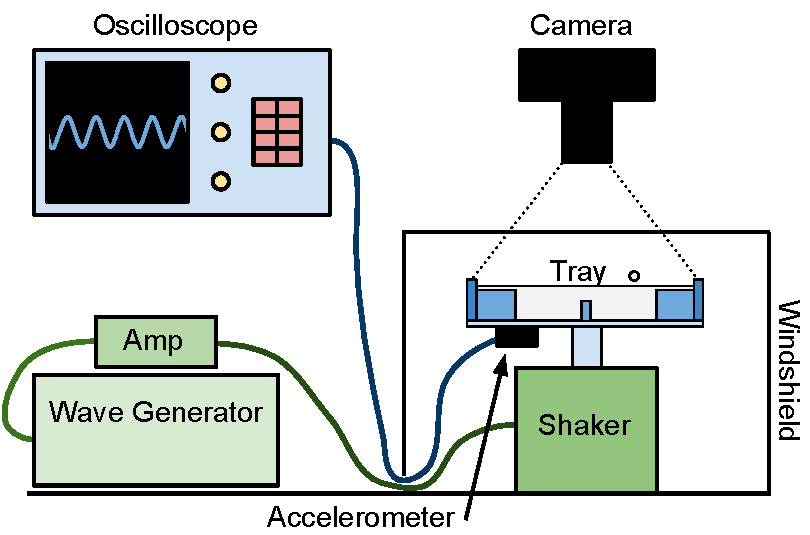
\includegraphics[scale=0.8]{Setup.pdf}
	\caption{The experimental setup. The amplified signal from the wave generator drives the shaker. The accelerometer generates a signal which is read by the oscilloscope. The windshield blocks disturbances to the experiment, while allowing the camera to document the trials.}
	\label{setup}
\end{figure}

\section{Materials}
The key components of this experiment are the shaker, the oil, and the tray. In this section I'll describe the specifics of the big three, as well as some of the additional components used in data collection. 

\subsection{Tray}
The tray was made of plastic parts machined by the (MODEL NUMBER?) laser cutter. They were then glued together with GLUE?. The tray's design guides the droplet and creates smooth droplet trajectories. The tray schematic is shown in \refFig{tray}. 

\begin{figure}[h!]
	\centering
	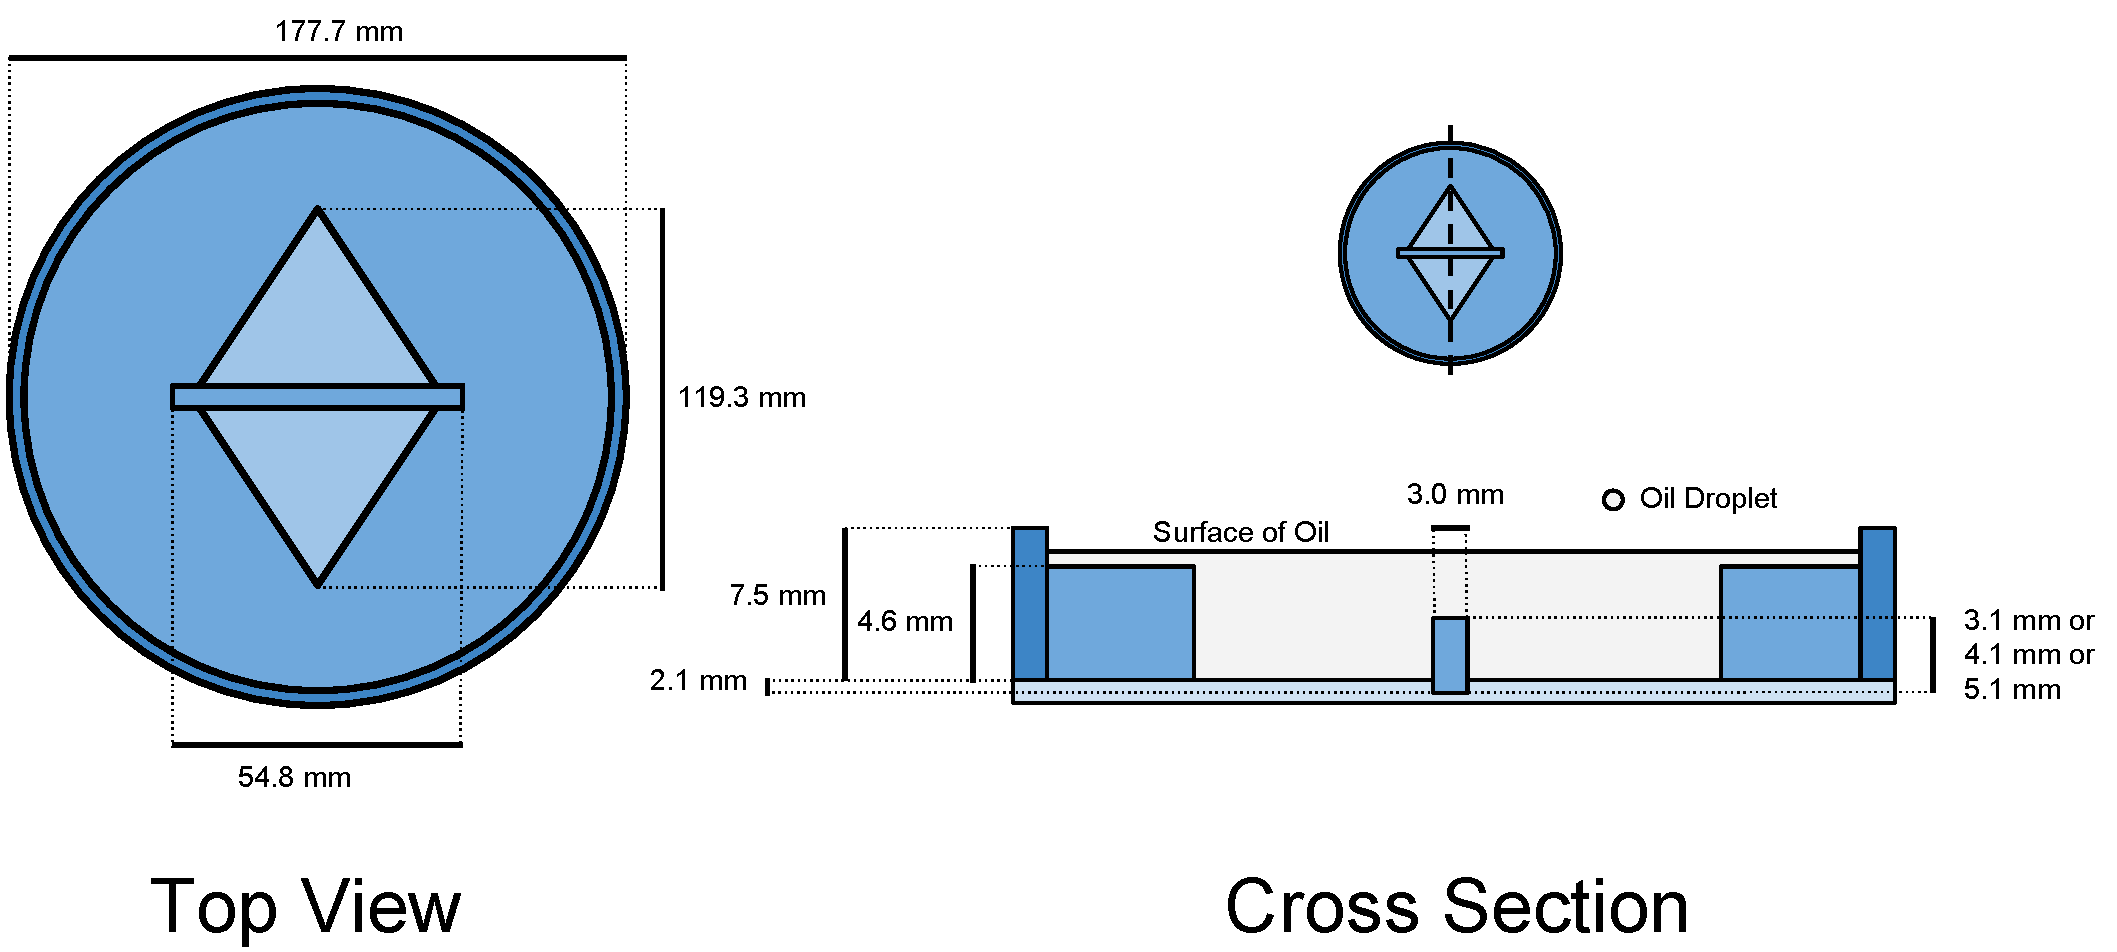
\includegraphics[scale=0.48]{Tray.pdf}
	\caption{The specifications of the tray design. The top view (left) highlights the main elements in the tray, while the cross section (right) illustrates the topography of the tray.}
	\label{tray}
\end{figure}

A thin layer of oil spills over the constraining rhombus shape. As long as the layer is thin enough, the droplet will remain in the rhombus container, but the waves will continue to propagate unimpeded. This gives the waves time to decay, and means that the droplets motion isn't chaotically affected by reflections of previous waves and is instead guided by the unreflected waves. 

The rhombus shape serves to steer the droplet into a perpendicular collision with the barrier. This works because the droplet will pin-ball its way into the acute corner of the rhombus, and will shoot out in a straight line, directly towards the barrier.  (FIGURE of pinballing droplet?)

I designed my experiment to test barriers of three different heights: $2.75~\mathrm{mm}$, $3.0~\mathrm{mm}$, and $3.25~\mathrm{mm}$, measured from the bottom of the rhombus. A thin barrier of plastic made by the laser cutter has the tendancy to bend and warp over time. The solution to this problem was to make these barriers taller than the specified heights, and create an cut-out in the rhombus so they could be inserted. The barrier cut-outs were deep enough to exactly counter the added height of the barrier, so the barriers still had (when measured from the surface of the rhombus) heights of $2.75~\mathrm{mm}$, $3.0~\mathrm{mm}$, and $3.25~\mathrm{mm}$. This also solved the problem of fixing the barriers in place, but still making them easily removable. These heights were chosen because they allowed for both passage over and blockage by the barriers. At the lowest heights, most droplets will cross over, where as taller barriers will block most droplets. 


The bottom of the tray was painted black in order to provide contrast, which allows the droplet to be more easily tracked by eye and by camera.

\subsection{Silicon Oil}
    The silicone oil used in this experiment had a viscosity of 20 cSt (the thickness is a little closer to water than olive oil) obtained from Clearco Products Co., Inc. (CAS No: 63148-62-9). The 20 cSt viscosity of Bush's group was used (over the 50 cSt viscosity of Couder's) because it has a larger walking regime than at other viscosities. The tray requires about x amount of fluid.
    
    It is of vital importance to keep the oil as clean as possible because it keeps the droplet bouncing for longer. This means protecting both from particulate matter that is already in the tray and from the particulate matter that might float on to the surface of the oil. Contamination can be minimized by cleaning the tray before pouring the oil in.
    
\subsection{Shaker}
    To shake the tray, we used a mechanical wave driver made by Pasco Scientific, model SF-9324. This shaker was designed to drive a string or an elastic cord, not a ~200 gram tray with oil inside, which was probably at the limit of what the shaker can handle. 
            
\subsection{Accelerometer}  
    Knowing the tray's acceleration allows us to characterize the behavior of our system using \refFig{regime}. To measure acceleration, we attached an ADLX 326 triple axis accelerometer to the bottom of the tray. The method of attachment was screws, since it provided a much firmer yet more removable hold than tape or glue. The accelerometer has a range of $\pm$16$g$, perfect for measuring the accelerations in our setup, which average about 5$g$'s. 
      
      The signal from the z-axis of the accelerometer was output directly into the oscilloscope. For the vibrating tray, the output was approximately sinusoidal (as expected). The spec sheet for the accelerometer indicates that the sensitivity can be translated to $57 \pm 6~\mathrm{mV/g}$. 

\subsection{Waveform Generator and Amplifier}
    The shaker was driven with the Agilent Arbitrary Waveform Generator model 33210, which was controlled digitally and thus created consistent waves.  
       
    Adding a Lepai LP2020A+ digital amplifier to the wavefunction generator meant the amplitude of the tray could be precisely controlled.   
    
\subsection{Windshield}
    A large, see-through cylinder (covered at one end) was manufactured by the laser cutter. When placed over the tray, it served the purpose of keeping the oil clean from particulate matter and preventing wind currents from influencing the motion of the walker.       
   
\subsection{Leveling Platform}
    A leveling platform was made out of wood, with three adjustments to adjust the tilt. This ensured that the tray was always flat. A level placed inside the tray (before the oil was added), ensured the 

\subsection{Camera}       
 

\section{Procedure}

\subsection{Finding the Walking Regime}

Before investigating the rate of tunneling using different barriers, a rough estimate of the walking regime at a frequency of $80~\mathrm{Hz}$ must be made to ensure correct behavior. A ``map" similar to the one in \refFig{regime} will be made, but rather than looking at all of the different kinds of bouncing we will limit ourselves to only the walking regime. Reproducing this figure allows us to find the parameters that are specific to our unique system, which could have slightly different height, tray, oil, and shaker configurations than those used in the literature. 

Droplet size is measured using a recorded video of the walking droplet in motion. By comparing the number of pixels making up the diameter of the droplet (unknown measurement) to the number of pixels making up the diameter of the tray (known measurement), we can estimate the ``length" of each pixel, and thus find the diameter of the droplet in centimeters. 

Driving acceleration values are measured by the accelerometer and displayed by the oscilloscope. 

To ensure that every trial has the same oil depth, we must measure the volume of the oil before filling the tray. Knowing the volume of the tray and of each barrier, we can get a value for the oil depth without interfering with the system. 

\subsection{The Experiment}

Tunneling was examined for three different barrier heights. At each height (and at a constant frequency of 80 Hz and constant driving acceleration), a string of continuous collisions were filmed with the camera. From this data, a fixed base tunneling ``probability" was calculated, which provides the most simplistic analysis of this system. 

The tray is designed such that most of the droplet's collisions with the barrier occur ``head on" (i.e. perpendicular to the length of the barrier), but not all collisions unfold ideally. A more involved analysis in \textit{Tracker} requires looking at the component of velocity of the droplet perpendicular to the length of the barrier, and determining the probability of tunneling given this value. Since not all collisions in the simplistic analysis occur at the same velocity, this method allows for a more methodical analysis of the phenomena. 
